\documentclass[a4paper,10pt]{article}
\usepackage{beamerarticle}
\usepackage[T1]{fontenc}
\usepackage[french]{babel}
\usepackage[utf8]{inputenc}
\usepackage{listings}
\usepackage{color}
\usepackage[pdftex,colorlinks=true,urlcolor=blue]{hyperref}
\usepackage{graphics}
\usepackage{graphicx}
\usepackage{ifthen}
\usepackage{fullpage}
\usepackage{times}
\usepackage{fancybox}
\usepackage[english]{qcm}

\renewcommand{\normalfont}{\sffamily} % Pour avoir de "l'arial"
\answerstitle{}

\begin{document}

\begin{center}
  \begin{Large}
    Grundlagen den Programmierung\\
    Revision Quizz\\
  \end{Large}
\end{center}

%\ifbook{

}

\ifslide {

  \begin{frame}{About me...}
    \begin{columns}

    \begin{column}[l]{.3\textwidth}
      \begin{center}
        \includegraphics[height=120px]{../img/rpe.jpg}
      \end{center}
    \end{column}

    \begin{column}[r]{.7\textwidth}
      \begin{block}{Romain PELISSE}
        \begin{itemize}
          \item \textbf{Middleware Consultant} at \mylink{http://redhat.com}{Red Hat} (2011)
          \begin{itemize}
            \item Architecte Middleware JBOSS
            \item Red Hat Linux Technician
          \end{itemize}
          \item Committer \mylink{http://pmd.sourceforge.net/}{PMD} and \mylink{http://xradar.sourceforge.net/}{XRadar}
          \item Translation for \mylink{http://www.selenic.com/mercurial/wiki/index.cgi/TranslatingMercurial}{HgBook}
          \item Teach build technologies and OPP at \mylink{http://www.esme.fr/}{ESME Sudria}
        \end{itemize}
      \end{block}
    \end{column}
   \end{columns}
 \end{frame}

 \section{Foreword}

 \begin{frame}
   \begin{block}{Some pratical details}
     \begin{itemize}
       \item I have previous experience in teaching, but to \textbf{technical} people or student
       \begin{itemize}
         \item ... so \textit{stop} me, if I go too fast !
       \end{itemize}
       \item I'm French, but I teach in \textbf{English} because my \textit{Deutsch ist schrecklich}
       \item Session last 3 hours, and are divided into:
       \begin{itemize}
         \item 15 minuten: small MCQ (Multiple choice questionnaire), starting next week
         \item ~1 hour
         \item 30" break
         \item ~1 hour
         \item 15" buffer if we are late or need to go deeper
       \end{itemize}
       \item we are here to \textbf{interact}, not to get your ears used to crappy english spoken by
       French people...
     \end{itemize}
   \end{block}
  \end{frame}

  \begin{frame}
    \begin{block}{Sessions agenda}
       \begin{itemize}
         \item 14h00 bis 17h30 - Freitag 04.05 (1/7 - 3h)
         \item 14h00 bis 17h30 - Freitag 11.05 (2/7 - 3h)
         \item 14h00 bis 17h30 - Freitag 25.05 (3/7 - 3h)
         \item 14h00 bis 17h30 - Freitag 01.06 (4/7 - 3h)
         \item \textbf{14h00 bis 17h30 - Freitag 22.06 (5/7 - 3h)}
         \item 14h00 bis 17h30 - Freitag 29.06 (6/7 - 3h)
         \item 14h00 bis 17h30 - Freitag 13.07 (7/7 - 3h)
      \end{itemize}
    \end{block}

    \begin{block}{Be careful !}
      Those dates can changes (and some will probably) - always checkout on Moodle if a session has
      not been rescheduled
    \end{block}
  \end{frame}

  \begin{frame}
    \begin{block}{Goals}
      \begin{itemize}
        \item Basic understanding of how and why program
        \item Impact in \textbf{your} job
        \item Enhance your communication skills with technical people
      \end{itemize}
    \end{block}

    \begin{block}{Who are you ?}
      \begin{itemize}
        \item Quickly gives us an hint of you are and where you come from...
      \end{itemize}
    \end{block}
  \end{frame}

  % classe outline
  \section{How computer works ?}

  \begin{frame}
    \begin{center}
        What do you know about \textbf{how} a computer work ?
    \end{center}
  \end{frame}

  \begin{frame}
   \begin{center}
     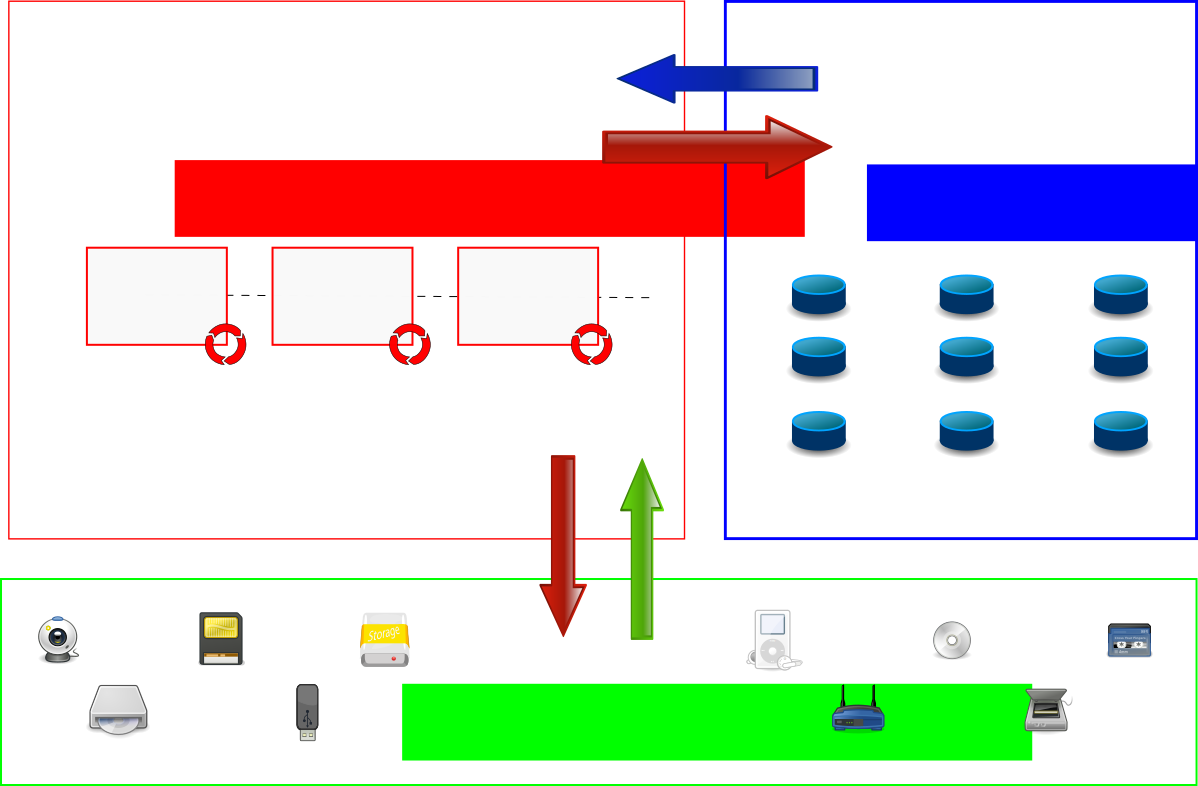
\includegraphics[scale=0.3]{img/cpu-schematics.png}
   \end{center}
  \end{frame}

  \begin{frame}
    \begin{center}
      \begin{itemize}
        \item What is an \textbf{operating system}(OS) ?
        \item Name a few OS names that you know of ?
        \item What does exactly an operating system ? What are its \textbf{responsabilities}?
      \end{itemize}
    \end{center}
  \end{frame}

  \begin{frame}{Role of an Operating System}
    \begin{center}
      \includegraphics[scale=0.3]{img/operating-system.png}
    \end{center}
  \end{frame}

  \begin{frame}{Speed of I/Os}
    \begin{center}
      \includegraphics[scale=0.3]{img/pyramid-io.png}
    \end{center}
  \end{frame}

  \section{Short history of IT}

  \begin{frame}{First era of IT: Mainframe and terminals}
    \begin{center}
      \includegraphics[scale=0.3]{img/mainframe-terminals.png}
    \end{center}
  \end{frame}

  \begin{frame}{Second era of IT: Clients and servers}
    \begin{center}
      \includegraphics[scale=0.3]{img/fat-clients.png}
    \end{center}
  \end{frame}

  \begin{frame}{Third era of IT: The Internet}
    \begin{center}
      \includegraphics[scale=0.3]{img/internet.png}
    \end{center}
  \end{frame}

  \begin{frame}{Data persistance}
    \begin{center}
      
\includegraphics[scale=0.3]{img/persistance.png}
    \end{center}
  \end{frame}

  \section{Java}

  \begin{frame}{Java}
    \begin{block}{What is Java ?}
      \begin{itemize}
        \item \textbf{programming} language
        \begin{itemize}
          \item "look-like" C code
          \item \textbf{Object Programming Oriented}
          \item strongly \textbf{structured}
        \end{itemize}
        \item operating system \textbf{independant}
        \item running within a \textbf{virtual machine}
        \item with automated memory collection
      \end{itemize}
    \end{block}

    \begin{center}
      \includegraphics[scale=0.2]{img/java-logo.jpg}
    \end{center}
  \end{frame}

  \begin{frame}{Java}
    \begin{block}{Compiling code....}
      \begin{itemize}
        \item What for ? What does it do ? What does it bring ?
        \item Must all languages be compiled ?
        \item If not, what is the point of compiled language ?
      \end{itemize}
    \end{block}
  \end{frame}

  \begin{frame}{Java}
    \begin{block}{The infamous Hello The World program...}
      \begin{itemize}
        \item What is this program ? What does it do ?
        \item Why does programmer always start by writing such a program ?
        \item Let's see how to implement such a program in Java...
      \end{itemize}
    \end{block}
  \end{frame}
}

%\input{mcf/session-02}

\begin{question}{
What is the point of using an IDE instead of a simple text editor when writing a program ?
}
  \false syntax coloration is nicer to look at
  \true  it speeds up the development and ensure the code produced is of quality
  \false an IDE ease working within a group of people on a the source code
  \false the IDE can compile and check if the code is valid
\end{question}

\begin{question}{
When trying to resolve a problem or a defect in a program, how should one try to find the root cause ?
}
  \false modify the code to add "print" statement describing the content of the variable
  \false look carefully at the code, to ascertain which part of it is not working properly
  \true use the debugger
  \false reboot your work station, and see if it does fix the problem
\end{question}

\begin{question}{
What is a \textbf{breakpoint} ?
}
  \false the defective part of a program
  \false a way to see interactively the content of a variable while a program is running
  \false a simple kind of variable
  \true a debugger mechanism to run the program up to a certain point
\end{question}

\begin{question}{
What is the purpose of an 'if' statement ?
}
  \false allow to easily repeat a piece of code
  \false assign a new value to a variable
  \true a simple form of control flow to direct the program to execute a certain portion of the code
  \false a mechanism to test if two variables have the same content
\end{question}

\begin{question}{
Check the \textbf{invalid} statement about it:\\
\small{
  \texttt{
    if ( a == b ) \{ \\
      \vspace{4pt} System.out.println("a == b"); \\
    \} else \{  \\
      \vspace{4pt} System.out.println("a != b");  \\
    \}
  }
}
}
  \false if the content of the variable 'a' and 'b' are the same, "a == b" is printed on the screen
  \false if the content of the variable 'a' and 'b' differs, "a != b" is printed on the screen
  \true if the content of the variable 'a' and 'b' differs, "a == b" is printed on the screen
  \false if the content of the variable 'a' and 'b' are not the same, "a != b" is printed on the screen
\end{question}

\begin{question}{
What is the purpose of a 'for' statement ?
}
  \false a simple mechanism to assign a new value to a variable
  \true iterate over a piece of code a certain number of time
  \false test if a variable is 'true'
  \false allocate more memory to a variable
\end{question}

\begin{question}{
Look at the following piece of code and pick the \textbf{invalid} statement about it:\\
\small{
  \texttt{
    for ( int i = 0 ; i < 10 ; i++ ) \{ \\
      \vspace{4pt} System.out.println("current iteration is:" + i); \\
    \}
  }
}
}
  \false the statement 'i++' is just an abbreviation for 'i = i + 1'
  \false at some point, this program will print "current iteration is:8"
  \false the value of the variable 'i' will be, at start, 0
  \true at some point, this program will print "current iteration is:10"
\end{question}

\begin{question}{
What is the purpose of a 'while' statement ?
}
  \false test if an operation returns true
  \false allocate more memory to a variable
  \true iterate over a piece of code until a certain condition is no longer verified (no longer
  returns 'true')
  \false it's a short cut to write an 'if' statement and 'for' statement
\end{question}

\begin{question}{
Look at the following piece of code and pick the \textbf{invalid} statement about it:\\
\small{
\texttt{
    int[] array = \{ 1,5,4,-6,7,9 \}; \\
    int i = 0; \\
    while ( array[i] > 0 ) \{ \\
      \vspace{4pt} System.out.println("Array[:" + i + "] = " + array[i]); \\
      \vspace{4pt} i++; \\
    \}
}
}
}
  \false this code will print 1,5,4
  \true this code will print all the values of the array
  \false 'array[i]' will access the value of the array stored at the position equals to the value of 'i'
  \false The '-6' will never be printed on the screen
\end{question}

\begin{question}{
In the following statements regarding functions, check the one which is \textbf{invalid}:
}
  \false reuse code easily
  \false make code easier to read
  \true implements a functionality (feature) of the program
  \false hide complexity
\end{question}

\begin{question}{
Which of the following item is \textbf{not} a part of a function:
}
  \false the return type
  \false the arguments
  \false the function body
  \true an if statement
\end{question}


\end{document}
